\chapter{テスト分析でのばらつき傾向とテストケース抜け漏れへの影響}\label{chap:3}
本章では,前章で述べた課題を更に分析するためにおこなった予備実験の結果を述べる.
実験では,被験者に対して,テストベースを与えてテスト分析を実施してもらい,その後,テスト分析手法の知識を与えた上で再度テスト分析をしてもらい,実験結果から,ルールがない状態でのテスト分析結果にはばらつきがあること,また,2章で説明をしたテストカテゴリベースドテストによるルールを与えることによる変化を調査する.

\newpage
\section{予備実験の目的} \label{sec:3-1}
2.4節の「テストカテゴリベースドテスト」にて示した実験では,分析手法を適用したグループが,導入していないグループよりも抜け漏れが少なく重複も少ない結果となった.
しかし,実験データは1組のみであり,傾向を見るためには不十分である.
テスト分析手法を適用する前のテスト分析での結果のばらつきの傾向,及びばらつきの傾向と分析手法を適用後の結果との相関をより多くのデータで調べることを目的に予備実験を行った.
実験はワークショップを通じてグループ単位2回,個人単位1回行なった.
\begin{description}
  \item[グループ単位①] 製造メーカーの同一製品開発チームのメンバーを4〜5人にグルーピングして実施(6サンプル収集)
  \item[グループ単位②] オープンな研修にて,別々の企業の参加者を4〜5人にグルーピングして実施(2サンプル収集)
  \item[個人単位①] テスト技術者コミュニティ主催のワークショップを通じて実施(57サンプル)
\end{description}

\newpage
\section{グループ単位の実験}
\subsection{実験の概要}
グループ単位の実験は2回行った.
両方とも4時間のワークショップを通じて実施した.

ワークショップの進め方を,図~\ref{fig:D-3-ExparimentAbst1}に示す.最初に,テスト開発プロセスを説明する.その後,演習に使うテストベースを示し,参加者に各自の考えに基づき,2.4.5節の実験と同様に「テスト分析の作業Step3:テストカテゴリを使った仕様項目と期待結果の選択」を実行してもらう.
その後,4〜5名の参加者をランダムにグルーピングし,グループ内で各自のテスト分析の結果をグループの回答としてまとめる.

最初の分析結果のまとめが終わり,全出席者のが各グループの分析結果を理解した後,テストカテゴリを用いたテスト分析手法と実施手順を説明して,手法の手順に沿って再度テスト分析を参加者が各自で実施する.
その後は最初の分析結果同様にグループの回答をまとめる.

解答例と同じだけの仕様項目を特定できれば網羅的にテスト分析ができているとする.
そのうえで,同一グループに対するテスト分析手法の知識を与える前と,知識を与えた後のグループ回答を実験のデータとして利用した.
\begin{figure}[h]
\begin{center}
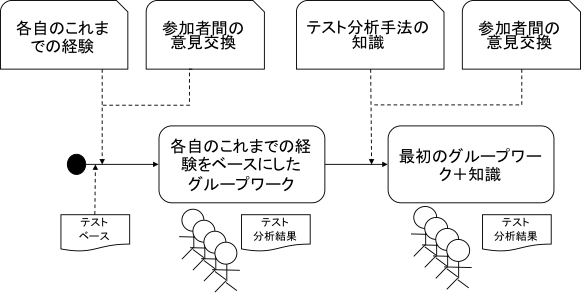
\includegraphics[width=10cm]{./image/D-3-ExparimentAbst1.png}
\caption{演習の前提条件の変化}
\label{fig:D-3-ExparimentAbst1}
\end{center}
\end{figure}

\subsection{実験の題材}
実験の題材は2種類用意した.
[グループ単位①]では,音楽再生機器を演習題材にした.フィーチャーセットはボリュームコントロールを対象にした.
これは2.4.5節で行なった実験と同じ演習題材である.
[グループ単位②]では,フライト予約Webシステムを演習題材にした.フィーチャーセットは新規フライト予約である.
テストベースとなる仕様書として,両方とも12枚のパワーポイントのスライドを用意している.
講師側が用意した解答例である,テスト分析で特定すべきテスト条件の一覧を表~\ref{tab:D-3-ensyu1}と表~\ref{tab:D-3-ensyu2}に示す.

% Table generated by Excel2LaTeX from sheet 'Sheet1'
\begin{table}[htbp]
  \scriptsize
  \centering
  \caption{音楽再生機器の講師解答例}
    \begin{tabular}{|l|l|p{13em}|p{18em}|}
    \hline
    \multicolumn{1}{|p{8em}|}{\textbf{論理的機能構造}} & \multicolumn{1}{p{14em}|}{\textbf{テストカテゴリ}} & \textbf{仕様項目} & \textbf{期待結果/確認内容} \bigstrut\\
    \hline
    \multicolumn{1}{|p{8.665em}|}{\textbf{対向機入力}} & \multicolumn{1}{p{14.085em}|}{\textbf{対向機入力}} & \textbf{--} & \textbf{--} \bigstrut\\
    \hline
    \multicolumn{1}{|p{8.665em}|}{\textbf{ボタン}} & \multicolumn{1}{p{14.085em}|}{\textbf{ボタン}} & \textbf{・キューイング} & \textbf{・早押ししたとき無視すること} \bigstrut\\
    \hline
    \multicolumn{1}{|p{8.665em}|}{\textbf{音声出力}} & \multicolumn{1}{p{14.085em}|}{\textbf{音声出力}} & \textbf{・ボリューム上限下限を知らせるビープ音} & \textbf{ビープ音が押下に対して1回なること} \bigstrut\\
    \hline
    \multicolumn{1}{|p{8.665em}|}{\textbf{LED点灯}} & \multicolumn{1}{p{14.085em}|}{\textbf{LED点灯}} & \textbf{--} & \textbf{--} \bigstrut\\
    \hline
    \multicolumn{1}{|p{8.665em}|}{\textbf{音量}} & \multicolumn{1}{p{14.085em}|}{\textbf{音量}} & \textbf{・音量調節} & \textbf{・ボタン押下でボリュームが上下すること} \bigstrut\\
    \hline
    \multicolumn{1}{|p{8.665em}|}{\textbf{対向機操作}} & \multicolumn{1}{p{14.085em}|}{\textbf{対向機操作}} & \textbf{-} & \multicolumn{1}{r|}{} \bigstrut\\
    \hline
    \multicolumn{1}{|l|}{\multirow{2}[2]{*}{\textbf{設定保存}}} & \multicolumn{1}{l|}{\multirow{2}[2]{*}{\textbf{設定保存}}} & \textbf{・デフォルト値} & \textbf{・ボリュームを変更させてリセットするとデフォルト値に戻ることで確認} \bigstrut[t]\\
          &       & \textbf{・音量調節の保存} & \textbf{・PowerON後前回Offした際の結果と同じ音量がでることを確認する} \bigstrut[b]\\
    \hline
    \multicolumn{1}{|p{8.665em}|}{\textbf{ヘッドセット状態遷移}} & \multicolumn{1}{p{14.085em}|}{\textbf{ヘッドセット状態遷移}} & \textbf{・状態により音量調節アクションを受け付ける/受け付けない} & \textbf{・再生中、通話中以外音量調節ボタンを無視する} \bigstrut\\
    \hline
    \multicolumn{1}{|p{8.665em}|}{\textbf{対向機への反映}} & \multicolumn{1}{p{14.085em}|}{\textbf{対向機への反映}} & \textbf{・対向機のボリューム値への影響} & \textbf{・ヘッドセットのボリュームを変更したあと、対向機のボリュームが変更していないことで確認} \bigstrut\\
    \hline
    \multicolumn{1}{|l|}{\multirow{2}[2]{*}{\textbf{設定情報の共有}}} & \multicolumn{1}{l|}{\multirow{2}[2]{*}{\textbf{設定情報の共有}}} & \textbf{・複数のPSKEYの設定影響} & \textbf{・通話と再生で交互に音量を調節した際に互いに影響を受けないこと} \bigstrut[t]\\
          &       & \textbf{・他の処理で音量設定の削除} & \textbf{・初期化、リセットで初期値に戻ることを確認} \bigstrut[b]\\
    \hline
    \end{tabular}%
  \label{tab:D-3-ensyu1}%
\end{table}%

% Table generated by Excel2LaTeX from sheet 'Sheet1'
\begin{table}[htbp]
  \scriptsize
  \centering
  \caption{フライト予約システムの講師解答例}
  \begin{tabular}{|l|l|p{13em}|p{18em}|}
  \hline
    \multicolumn{1}{|p{8.665em}|}{\textbf{論理的機能構造}} & \multicolumn{1}{p{14.085em}|}{\textbf{テストカテゴリ}} & \textbf{仕様項目} & \textbf{期待結果/確認内容} \bigstrut\\
    \hline
    \multicolumn{1}{|l|}{\multirow{8}[2]{*}{\textbf{画面入力}}} & \multicolumn{1}{l|}{\multirow{8}[2]{*}{\textbf{画面入力}}} & \textbf{・画面表示内容} & \textbf{・画面仕様書に沿ったレイアウトであること} \bigstrut[t]\\
          &       & \textbf{・年、月、日の入力範囲チェック} & \textbf{・入力フィールド/ボタンの制御が仕様どおりであること} \\
          &       & \textbf{・入力桁数チェック} & \textbf{・Min日以降Max日が入力できること} \\
          &       & \textbf{・型チェック} & \textbf{・フライト予約可能日以前の入力はクリアされること} \\
          &       & \textbf{・うるう年判定、末日判定} & \textbf{・桁数/文字数のチェックをすること} \\
          &       & \textbf{・出発地と到着地の組合せ} & \textbf{・型(文字,数値)のチェックをすること (仕様記述なし)} \\
          &       & \multicolumn{1}{r|}{} & \textbf{・うるう年、末日判定のチェックをすること} \\
          &       & \multicolumn{1}{r|}{} & \textbf{・同じ出発地と到着地を選択できないこと} \bigstrut[b]\\
    \hline
    \multicolumn{1}{|p{8.665em}|}{\textbf{ボタン操作}} & \multicolumn{1}{p{14.085em}|}{\textbf{ボタン操作}} & \textbf{・画面遷移} & \textbf{・画面仕様書に沿った画面の遷移ができること} \bigstrut\\
    \hline
    \multicolumn{1}{|l|}{\multirow{5}[2]{*}{\textbf{結果表示}}} & \multicolumn{1}{l|}{\multirow{5}[2]{*}{\textbf{結果表示}}} & \textbf{・プログレスバー/登録完了メッセージ} & \textbf{・登録中と登録後の表示が正しいこと} \bigstrut[t]\\
          &       & \textbf{・注文不成立メッセージ} & \textbf{・状況に合ったメッセージが出ること} \\
          &       & \textbf{・金額計算表示} & \textbf{・表示がフィールドに収まること} \\
          &       & \textbf{・注文番号} & \textbf{・ 同上} \\
          &       & \textbf{・フライト情報} & \textbf{・ 同上(検索画面、登録画面で確認)} \bigstrut[b]\\
    \hline
    \multicolumn{1}{|p{8.665em}|}{\textbf{帳票出力}} & \multicolumn{1}{p{14.085em}|}{\textbf{帳票出力}} & \textbf{--} & \textbf{--} \bigstrut\\
    \hline
    \multicolumn{1}{|l|}{\multirow{4}[2]{*}{\textbf{計算}}} & \multicolumn{1}{l|}{\multirow{4}[2]{*}{\textbf{計算}}} & \textbf{・合計額の計算} & \textbf{・クラス単価×人数となること} \bigstrut[t]\\
          &       & \textbf{・登録時の採番} & \textbf{・直前のNo+1となること} \\
          &       & \textbf{・チケット在庫の計算} & \textbf{・在庫数から購入数をマイナスし0以下にできない} \\
          &       & \multicolumn{1}{r|}{} & \textbf{(購入キャンセルの在庫数反映はここでは見ない)} \bigstrut[b]\\
    \hline
    \multicolumn{1}{|p{8.665em}|}{\textbf{検索}} & \multicolumn{1}{p{14.085em}|}{\textbf{検索}} & \textbf{・フライト検索結果} & \textbf{・検索条件(and)で該当するフライトが検索されること} \bigstrut\\
    \hline
    \multicolumn{1}{|p{8.665em}|}{\textbf{登録、更新、削除}} & \multicolumn{1}{p{14.085em}|}{\textbf{登録、更新、削除}} & \textbf{・フライトの登録} & \textbf{・フライトが登録が出来ること} \bigstrut\\
    \hline
    \multicolumn{1}{|l|}{\multirow{3}[2]{*}{\textbf{反映}}} & \multicolumn{1}{l|}{\multirow{3}[2]{*}{\textbf{反映}}} & \textbf{・「既存注文開く」への反映} & \textbf{・検索条件(and)で検索されること} \bigstrut[t]\\
          &       & \textbf{・「注文件数グラフ」への反映} & \textbf{・注文件数がプラスされること} \\
          &       & \textbf{・「注文履歴」への反映} & \textbf{・全ての状況(登録)が書き込まれること} \bigstrut[b]\\
    \hline
    \multicolumn{1}{|l|}{\multirow{2}[2]{*}{\textbf{エラー処理}}} & \multicolumn{1}{l|}{\multirow{2}[2]{*}{\textbf{エラー処理}}} & \textbf{・登録時にチケット在庫なし} & \textbf{・エラーになること  (仕様記述なし)} \bigstrut[t]\\
          &       & \textbf{・注文挿入中の強制終了} & \textbf{・ロールバックすること (仕様記述なし)} \bigstrut[b]\\
    \hline
    \end{tabular}%
  \label{tab:D-3-ensyu2}%
\end{table}%

\subsection{テスト分析手法適用前のテスト分析の結果}

ルールがない状態でのテスト分析結果のばらつきについて,実験による典型的な4パターンのテスト分析結果を図 ~\ref{fig:D-3-Fig1-1}から図 ~\ref{fig:D-3-Fig1-4}で示す.
\begin{enumerate}
\item CS1 と CS2:両方ともテスト対象の入力フィールドを行タイトルに列挙している.しかしながら列名と表の内容が異なっている.
\item CS3: 表の中に記載されている各列,アクションとパラメータと期待結果などが独立しているため,それぞれの間の関連を特定できない.
\item CS4: テスト対象の状態が列名として列挙されている.各状態で取りうるパラメータと値が表の中に記載されている.
\end{enumerate}

この結果は複数の個人のテスト分析が,それぞれ複数の結果に到達することを示している.
複数の結果とは,テスト分析を通して特定したテスト条件にばらつきがあることを意味している.
テスト分析が多くの人たちで行われるときには,テスト条件の重複,もしくは完全に抜け落ちるといった可能性が非常に高くなると考えられる.
仮説として,テストカテゴリベースドテストの知識を与えることで,ルールが適用されるため,テスト条件の特定できる数が増加すると考えられる.

\begin{figure}[H]
\centering
\subfloat[テスト分析の事例:CS1]{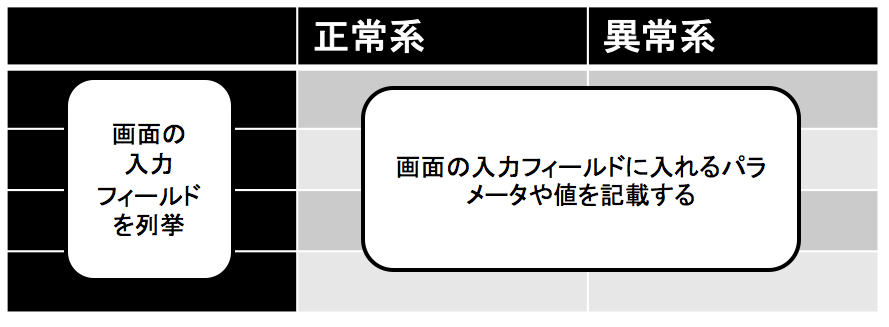
\includegraphics[clip, width=4in]{./image/D-3-Fig1-1.png}
\label{fig:D-3-Fig1-1}}
\\
\subfloat[テスト分析の事例:CS2]{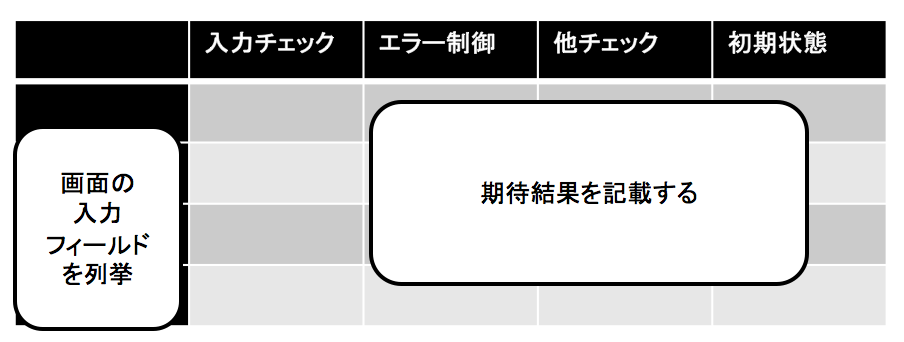
\includegraphics[clip, width=4in]{./image/D-3-Fig1-2.png}
\label{fig:D-3-Fig1-2}}
\\
\subfloat[テスト分析の事例:CS3]{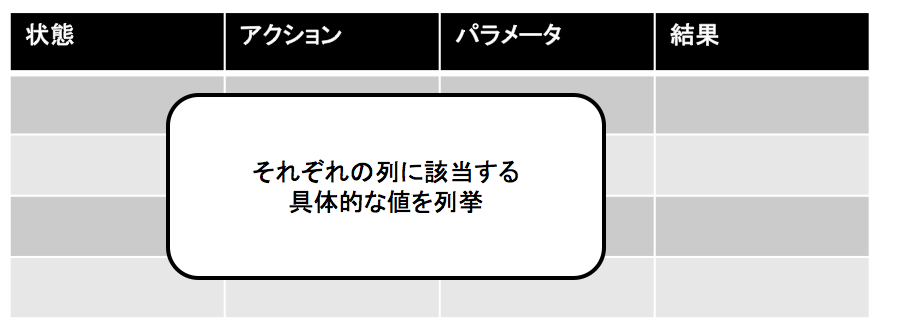
\includegraphics[clip, width=4in]{./image/D-3-Fig1-3.png}
\label{fig:D-3-Fig1-3}}
\\
\subfloat[テスト分析の事例:CS4]{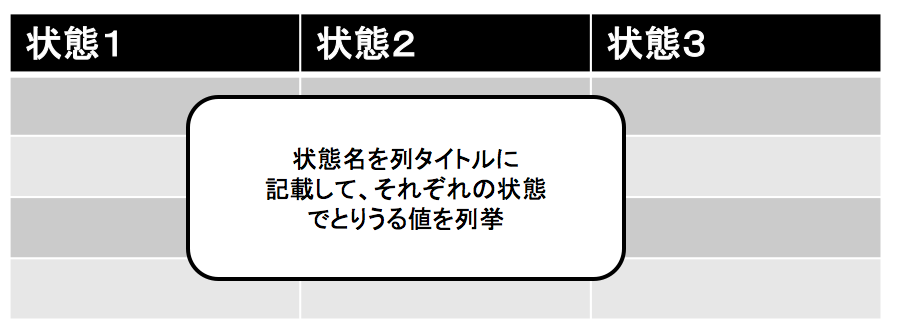
\includegraphics[clip, width=4in]{./image/D-3-Fig1-4.png}
\label{fig:D-3-Fig1-4}}
\caption{テスト分析の事例}
\label{fig:D-3-Fig1-1234}
\end{figure}


\subsection{1回目と2回目の検証実験結果の評価}
1回目,2回目の実験では,グループでの回答を実験結果として利用した.
1回目の実験は,組み込み開発を行なっている組織内での6チームの実験結果を収集し
2回目の実験結果ではオープンセミナーの参加者をグルーピングした2つの実験結果を収集したので,合計で8つの実験結果を収集した.
題材は,1回目の実験では音楽再生機器をテスト対象の$AS$にした.
2回目の実験では,飛行機予約システムをテスト対象の$AS$にした.
テストカテゴリベースドテストの知識をを与える前の演習結果と,テストカテゴリの知識を与えた後の演習結果とを比較した.
表~\ref{tbl:D-3-tbl3}は最初の演習結果のうちの1つの結果を比較した表である.

% Table generated by Excel2LaTeX from sheet '途中経過'
\begin{table}[htbp]
  \centering
  \caption{1回目の実験のチーム2(TM2)での比較結果 }
    \begin{tabular}{|l|r|r|r|r|}
    \hline
    \multirow{2}[4]{*}{テストカテゴリ} & \multicolumn{2}{c|}{期待結果数} & \multicolumn{2}{c|}{パラメータ数} \bigstrut\\
\cline{2-5}          & \multicolumn{1}{l|}{適用なし} & \multicolumn{1}{l|}{適用あり} & \multicolumn{1}{l|}{適用なし} & \multicolumn{1}{l|}{適用あり} \bigstrut\\
    \hline
    入力A   & \multicolumn{1}{l|}{N/A} & \multicolumn{1}{l|}{N/A} & \multicolumn{1}{l|}{N/A} & \multicolumn{1}{l|}{N/A} \bigstrut\\
    \hline
    \multirow{2}[4]{*}{変換A} & 1     & 1     & 3     & 3 \bigstrut\\
\cline{2-5}          & 0     & 1     & 0     & 3 \bigstrut\\
    \hline
    変換B   & 0     & 0     & 0     & 0 \bigstrut\\
    \hline
    サポートA & 0     & 0     & 6     & 0 \bigstrut\\
    \hline
    \multirow{2}[4]{*}{サポートB} & 0     & 0     & 0     & 0 \bigstrut\\
\cline{2-5}          & 0     & 0     & 0     & 0 \bigstrut\\
    \hline
    出力A   & 1     & 1     & 2     & 2 \bigstrut\\
    \hline
    出力B   & 0     & 0     & 0     & 0 \bigstrut\\
    \hline
    貯蔵A   & 0     & 1     & 0     & 1 \bigstrut\\
    \hline
    貯蔵B   & \multicolumn{1}{l|}{N/A} & \multicolumn{1}{l|}{N/A} & \multicolumn{1}{l|}{N/A} & \multicolumn{1}{l|}{N/A} \bigstrut\\
    \hline
    \multirow{2}[4]{*}{相互作用A} & 0     & 1     & 0     & 2 \bigstrut\\
\cline{2-5}          & \multicolumn{1}{l|}{N/A} & \multicolumn{1}{l|}{N/A} & \multicolumn{1}{l|}{N/A} & \multicolumn{1}{l|}{N/A} \bigstrut\\
    \hline
    合計    & 2     & 5     & 11    & 11 \bigstrut\\
    \hline
    \end{tabular}%
  \label{tbl:D-3-tbl3}%
\end{table}%


テストカテゴリベースドテストの知識を与える前にテスト分析をした結果は,図~\ref{fig:D-3-Fig1-1234}のようにばらつくので,ワークショップの後に講師が仕様項目の数を計算できるように仕様項目の分類をしている.

8つの実験結果を比較するために,表~\ref{tbl:D-3-tbl4}に示した評価レベルを設定した.

% Table generated by Excel2LaTeX from sheet 'Sheet1'
\begin{table}[htbp]
\footnotesize
  \centering
  \caption{評価レベルの定義}
    \begin{tabular}{|l|p{14em}|}
       \hline
    評価レベル & \multicolumn{1}{l|}{比較結果} \\
        \hline
     B    & リストしたテスト条件数は増加していない, かつ実験の期待結果よりも少ない.  \\
        \hline
    -     & リストしたテスト条件数は増加していない, しかしすでに期待結果と同数である.  \\
        \hline
    A     & リストしたテスト条件数は増加している, しかし実験の期待結果よりも少ない.   \\
       \hline
    A${}^\text{+}$    & リストしたテスト条件数は増加している, かつ実験の期待結果に達している. テスト条件の数は増加していない,.  \\
        \hline
    \end{tabular}%
  \label{tbl:D-3-tbl4}%
\end{table}%

検証実験にて収集した8つの評価結果を表~\ref{tbl:D-3-tbl5}に示す.

\begin{table}[htbp]
\footnotesize
  \centering
  \caption{8つのチームの検証実験の評価結果}
    \begin{tabular}{|l|l|l|l|l|l|l|l|l|}
    \hline
    \multicolumn{1}{|c|}{\multirow{2}[4]{*}{論理的機能構造}} & \multicolumn{8}{c|}{チーム} \bigstrut\\
\cline{2-9}          & TM1   & TM2   & TM3   & TM4   & TM5   & TM6 & TM7 & TM8 \bigstrut\\
    \hline
    変換  & B     & A     & B     & B     & B     & B & A     & A\bigstrut\\
    \hline
    入力 &  -     &   -     &   -    &   -    &   -    & -     & A     & B   \bigstrut\\
    \hline
    出力 & -     & -     & -     & -     & -     & A${}^\text{+}$ & A     & A \bigstrut\\
    \hline
    貯蔵 & -     & A${}^\text{+}$    & -     & A${}^\text{+}$    & A${}^\text{+}$    & -& A     & A  \bigstrut\\
    \hline
    サポート & B     & B     & B     & B     & B     & B& B     & A \bigstrut[t]\\
    \hline
    相互作用  & B     & A     & A     & A${}^\text{+}$    & A     & A${}^\text{+}$& B     & A \bigstrut[b]\\
    \hline
    \end{tabular}%
  \label{tbl:D-3-tbl5}%
\end{table}%

TM1からTM6までは最初の実験の結果である.
$AS$は音楽生成機器がであり,フィーチャセットはボリュームコントロールである.
この実験結果では,演習の解答例と同じだけのテスト条件を特定できたチームは0であった.
ただし,6チーム中5チームにおいて,列挙したテスト条件の数が増えている.
論理的機能構造の要素ごとの比較では,相互作用にて5チームの列挙数が増加している.
出力調整と貯蔵では,列挙数が増加したチーム以外は特定すべき仕様項目がすでに最初の演習で列挙できているため,効果があったかどうかはこの結果からは判断できない.
ただし,サポートでは全チームにて増加していないため,効果はなかった.

TM7とTM8は2回目の実験であり,$AS$はフライト予約システムであり,新規フライト予約がフィーチャセットである.
2回目の演習結果でも解答例と同じ数のテスト条件を特定したチームはいなかった.
ただし,2チーム全てにおいてテストカテゴリ内に列挙したテスト条件の数が増えている.
論理的機能構造の要素ごとの比較では,変換と出力調整と貯蔵にて2チームともにテスト条件の列挙数が増えた.
それ以外の要素では1チームのみが列挙数が増えた結果となっている.

全体的に定量的な向上が見られたが,特定のグループが著しく成長した,もしくは論理的機能構造の要素毎に特徴的な傾向は見出せなかった.
サンプルとなるデータ数が8つと少ないため,3回目の検証実験では,実験データ取得の方法を変更した.

\newpage
\section{3回目の検証実験からの考察}
\subsection{3回目の検証実験結果の評価} \label{sec:3-2}

3回目の検証実験では,グループ単位ではなく,各参加者の実施結果を収集した.
\begin{figure}[h]
\begin{center}
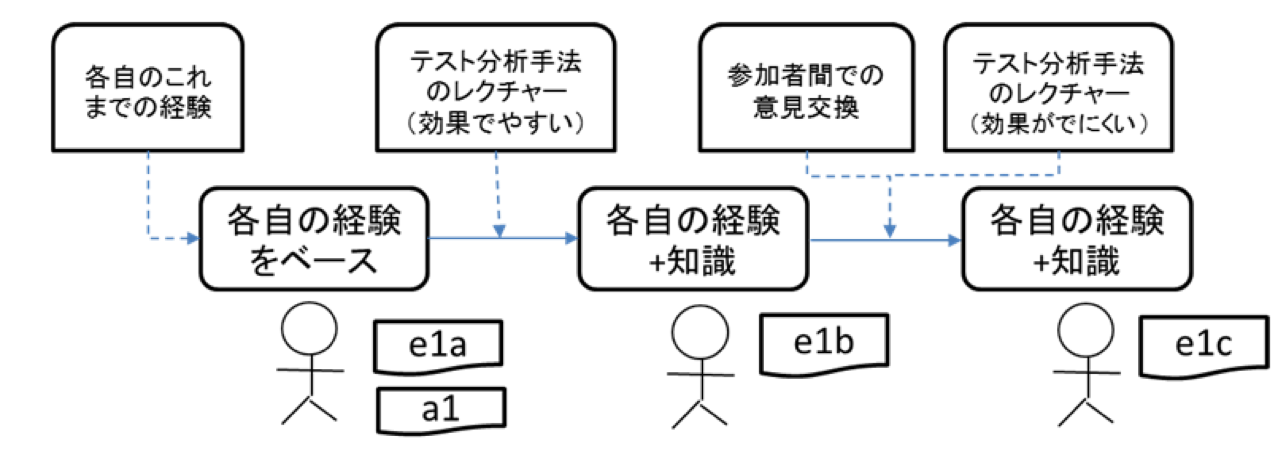
\includegraphics[width=10cm]{./image/D-3-Fig8.png}
\caption{e1aからe1cまでの演習の前提条件の変化}
\label{fig:D-3-Fig8}
\end{center}
\end{figure}
ワークショップを通して,図~\ref{fig:D-3-Fig8}のように,テスト分析手法を知らない状態での演習実施(1a),
一部分だけ説明した状態で演習実施(1b),
全てを説明した状態で演習実施を(1c)行い,各参加者の演習結果を実験データとして収集した.

テスト分析手法のレクチャーを2 回に分けた理由は, 前述したように手法の実施手順がデータフローを使った手順とそれ以外の手順に分けられるため, 2 段階にわけることがワークショップの参加者にとって知識習得が容易になるであろうという判断からである.

\begin{figure}[h]
\begin{center}
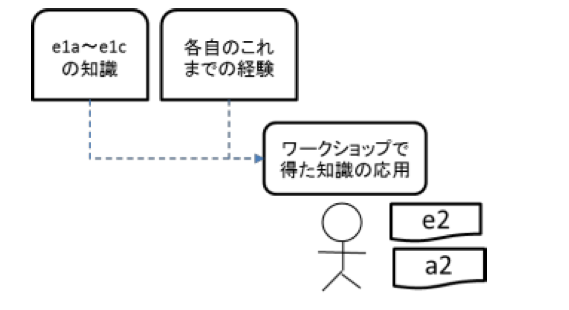
\includegraphics[width=10cm]{./image/D-3-Fig9.png}
\caption{e2 の演習の前提条件の変化}
\label{fig:D-3-Fig9}
\end{center}
\end{figure}
e2 では,図~\ref{fig:D-3-Fig9}のように,e1a からe3a までで行ったレクチャーと演習を通じて得た知識とスキルが別の題材で活用できることを確認する. e1a と比較することで, スキルが向上しているかを観察する.
%すべて説明した状態で演習実施(1c)を行い,各参加者の演習結果を実験データとして収集した.
このワークショップでは,57名分のIT技術者が参加した.
参加者の構成は図~\ref{fig:D-3-Fig6}と図~\ref{fig:D-3-Fig7}のとおりである.
年齢構成,業務領域ともに偏りがなく,産業界のサンプリングとして意味があると考える.
参加者の技術経験と,テスト技法の研修受講有無(テスト技法に関する知識習得)については, 記述式の調査紙にて確認を行った.

\begin{figure}[h]
  \begin{center}
  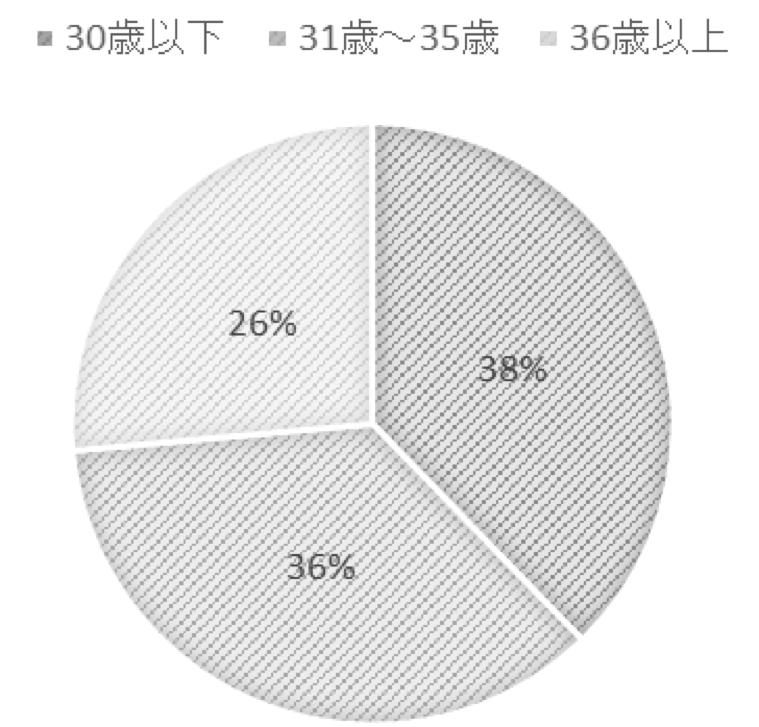
\includegraphics[width=10cm]{./image/D-3-Fig6.png}
  \caption{参加者の年齢分布}
  \label{fig:D-3-Fig6}
  \end{center}
   \end{figure}

   \begin{figure}[h]
  \begin{center}
  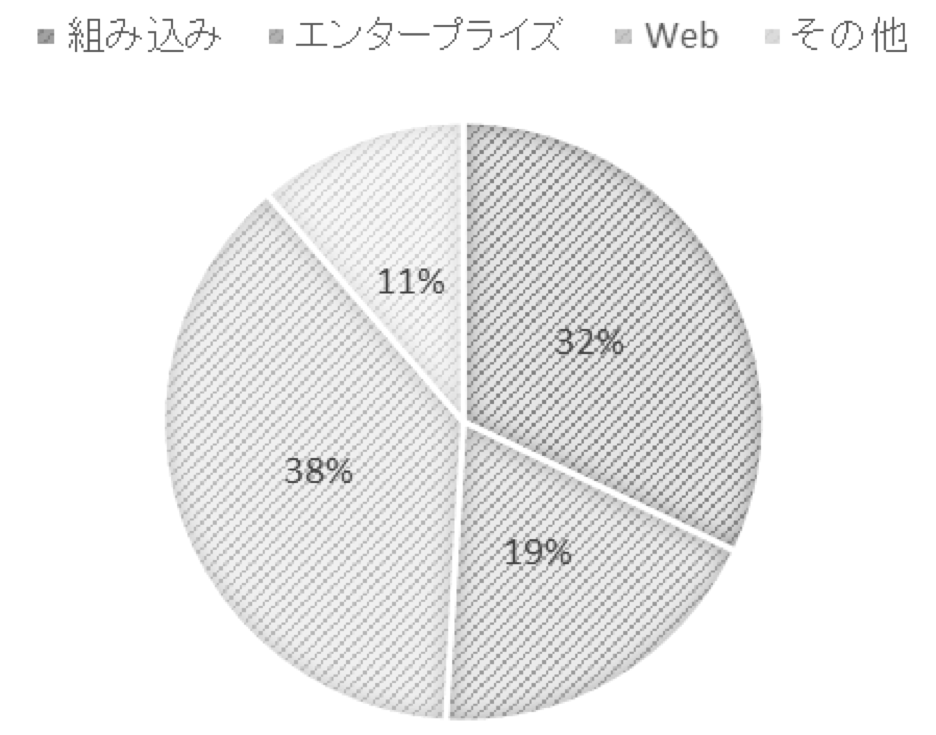
\includegraphics[width=10cm]{./image/D-3-Fig7.png}
  \caption{参加者の業務領域分布}
  \label{fig:D-3-Fig7}
  \end{center}
   \end{figure}

e1a,e1b,e1c,e2 の演習結果において,各参加者が特定できたテスト条件数 (回答数) を図~\ref{fig:D-3-Fig10}の箱ひげ図を用いて比較する.
図~\ref{fig:D-3-Fig10}のY軸は回答したテスト条件数を示し,X 軸は,各演習における回答数の分布を箱ひげ図で示している.

%箱ひげ図 %<図7 参加者あたりのテスト条件特定数>
\begin{figure}[htbp]
  \begin{center}
  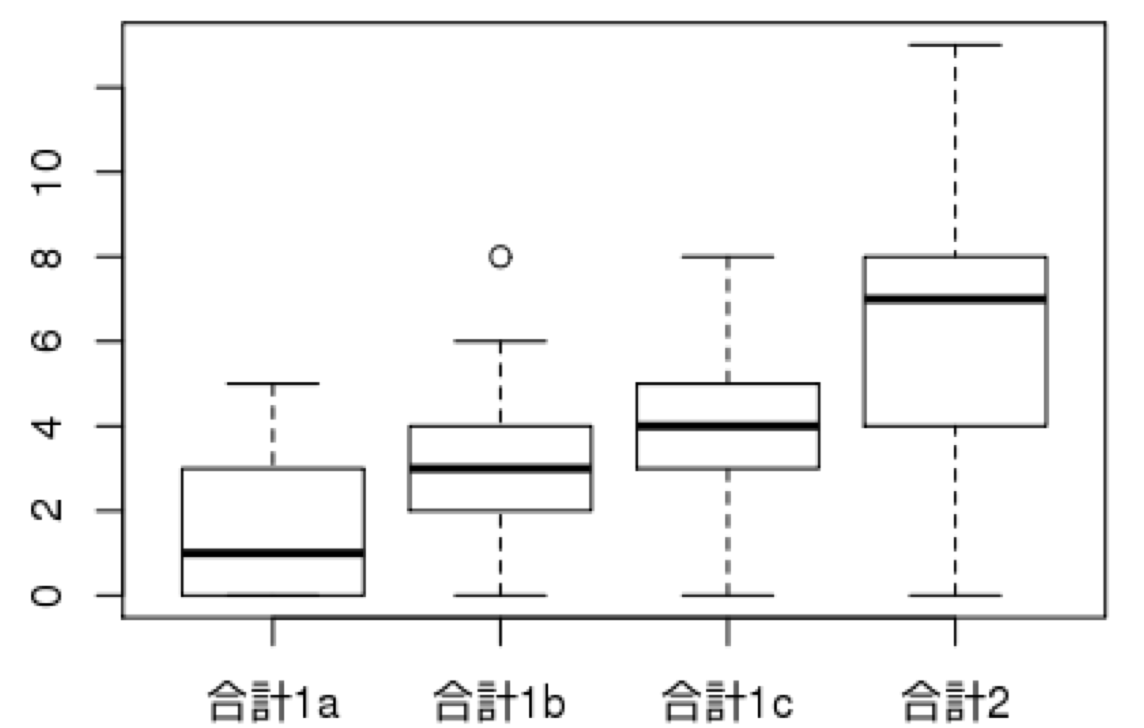
\includegraphics[width=10cm]{./image/D-3-Fig10.png}
  \caption{参加者あたりのテスト条件特定数}
  \label{fig:D-3-Fig10}
  \end{center}
\end{figure}

例えばe1aでは,最高点は5であり,中央値は1 であった.
正解数とした数は9なので,非常に低い値であった.
レクチャー後のe1bでは中央値が3,e1c では4,e2 では7 と,演習が進むごとに中央値が増えているので,テスト条件数を特定するスキルが向上したと考えられる.
ただし,e2 とそれ以外は演習題材が異なり,正解とした条件数が異なる(e2 は23 で,それ以外は9 である).
そのため,単純な数値の比較では不十分である.
正解とするケース数を100 とした箱ひげ図を図8 に示す.
%<図8 参加者あたりのテスト条件特定割合>
\begin{figure}[htbp]
  \begin{center}
  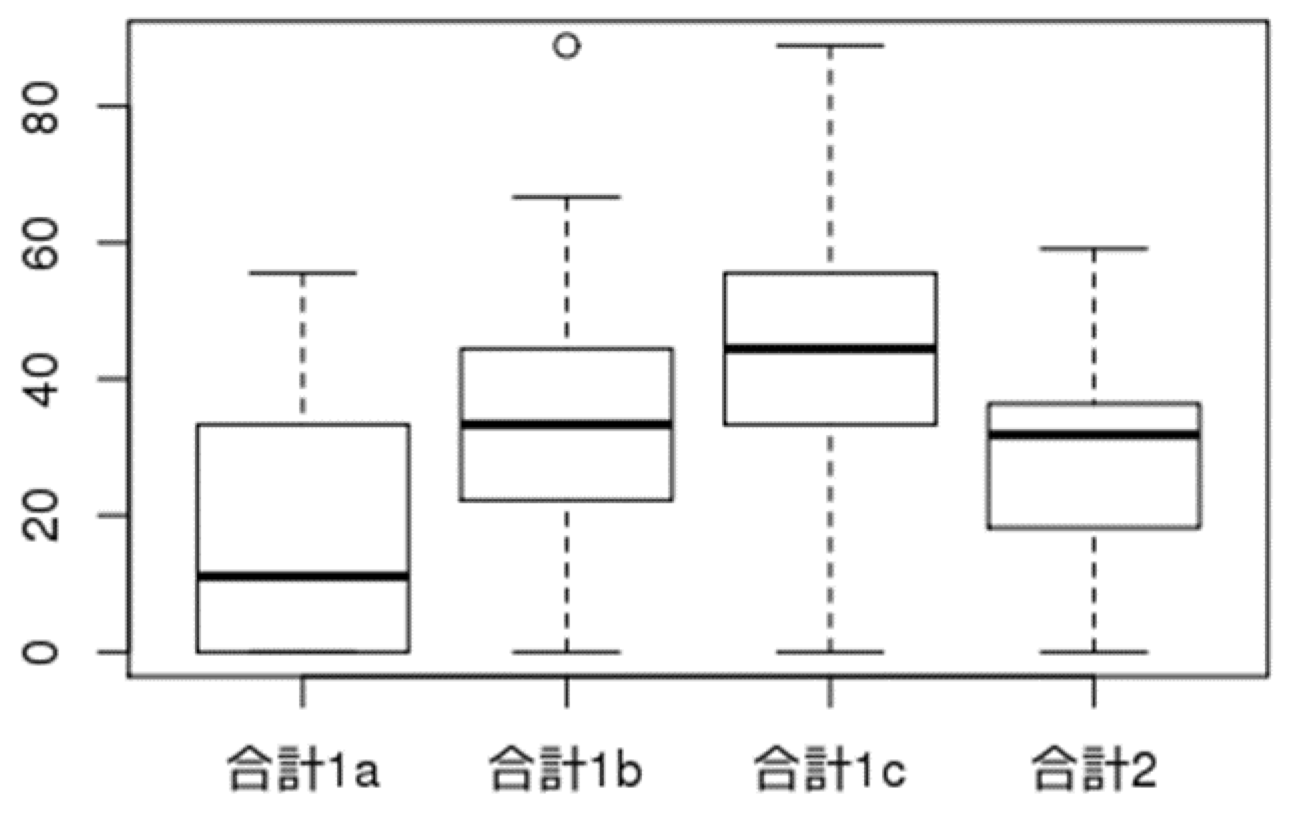
\includegraphics[width=10cm]{./image/D-3-Fig11.png}
  \caption{参加者あたりのテスト条件特定割合}
  \label{fig:D-3-Fig11}
  \end{center}
   \end{figure}

図~\ref{fig:D-3-Fig11}からは, e1a では約10% であったテスト条件の特定数の割合の中央値が,e2 では約40%まで向上したことが確認できる.
ただし,図~\ref{fig:D-3-Fig10}と図~\ref{fig:D-3-Fig11}からわかるように参加者全員のテスト条件特定数が一律に上がったわけではない.
効果があった部分とそうでない部分がどこであるかを調べるために,テスト条件ごとの特徴,および参加者の特徴でさらに分析をすすめた.

\begin{figure}[htbp]
  \begin{center}
  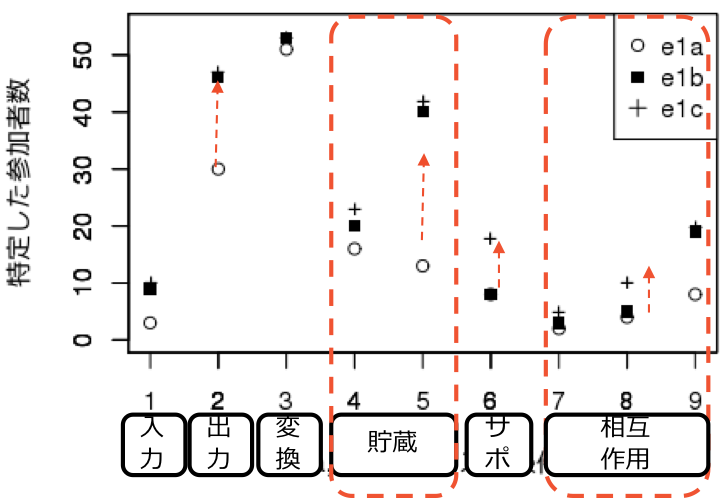
\includegraphics[width=7cm]{./image/D-3-Fig12-1.png}
  \caption{参加者あたりのテスト条件特定数}
  \label{fig:D-3-Fig12-1}
  \end{center}
\end{figure}
各参加者が特定できたテスト条件数 (回答数) を図\ref{fig:D-3-Fig12-1}のように論理的機能構造で分類して比較した.
図\ref{fig:D-3-Fig12-1}のY軸はテスト条件毎に解答できた参加者数を示し,X軸は,テスト条件を示している.
1a,1b,1c と進むにつれて,分析で特定できるテスト条件が増えていることがわかる.
テスト分析手法の知識を与えることで特に伸びたのは,出力と貯蔵に属するテスト条件であった.

\begin{table}[htbp]
  \centering
  \caption{e1a からe1c までの演習結果の変化表}
    \begin{tabular}{rrrrr}
    \hline
    \multicolumn{1}{|l|}{} & \multicolumn{1}{p{6em}|}{\textbf{論理的機能構造}} & \multicolumn{1}{p{6em}|}{\textbf{テストカテゴリ}} & \multicolumn{1}{p{6em}|}{\textbf{難しさ}} & \multicolumn{1}{p{6em}|}{\textbf{効果}} \bigstrut\\
    \hline
    \multicolumn{1}{|l|}{1} & \multicolumn{1}{p{6em}|}{入力調整} & \multicolumn{1}{p{6em}|}{ボタン} & \multicolumn{1}{p{6em}|}{難} & \multicolumn{1}{p{6em}|}{中} \bigstrut\\
    \hline
    \multicolumn{1}{|l|}{2} & \multicolumn{1}{p{6em}|}{出力調整} & \multicolumn{1}{p{6em}|}{音声出力} & \multicolumn{1}{p{6em}|}{中} & \multicolumn{1}{p{6em}|}{高} \bigstrut\\
    \hline
    \multicolumn{1}{|l|}{3} & \multicolumn{1}{p{6em}|}{変換} & \multicolumn{1}{p{6em}|}{音量} & \multicolumn{1}{p{6em}|}{易} & \multicolumn{1}{p{6em}|}{低} \bigstrut\\
    \hline
    \multicolumn{1}{|l|}{4} & \multicolumn{1}{l|}{\multirow{2}[4]{*}{貯蔵}} & \multicolumn{1}{p{6em}|}{設定保存1} & \multicolumn{1}{p{6em}|}{難} & \multicolumn{1}{p{6em}|}{中} \bigstrut\\
\cline{1-1}\cline{3-5}    \multicolumn{1}{|l|}{5} & \multicolumn{1}{l|}{} & \multicolumn{1}{p{6em}|}{設定保存2} & \multicolumn{1}{p{6em}|}{難} & \multicolumn{1}{p{6em}|}{高} \bigstrut\\
    \hline
    \multicolumn{1}{|l|}{6} & \multicolumn{1}{p{6em}|}{サポート} & \multicolumn{1}{p{6em}|}{状態遷移} & \multicolumn{1}{p{6em}|}{難} & \multicolumn{1}{p{6em}|}{中} \bigstrut\\
    \hline
    \multicolumn{1}{|r|}{7} & \multicolumn{1}{l|}{\multirow{3}[6]{*}{相互作用}} & \multicolumn{1}{p{6em}|}{対向機反映} & \multicolumn{1}{p{6em}|}{難} & \multicolumn{1}{p{6em}|}{低} \bigstrut\\
\cline{1-1}\cline{3-5}    \multicolumn{1}{|r|}{8} & \multicolumn{1}{l|}{} & \multicolumn{1}{p{6em}|}{設定情報共有1} & \multicolumn{1}{p{6em}|}{難} & \multicolumn{1}{p{6em}|}{中} \bigstrut\\
\cline{1-1}\cline{3-5}    \multicolumn{1}{|r|}{9} & \multicolumn{1}{l|}{} & \multicolumn{1}{p{6em}|}{設定情報共有2} & \multicolumn{1}{p{6em}|}{難} & \multicolumn{1}{p{6em}|}{中} \bigstrut\\
    \hline
    \multicolumn{5}{p{30em}}{難しさ 0-10難 11-25中 26-易} \bigstrut[t]\\
    \multicolumn{5}{r}{効果  0-10低 11-25中 26-高} \\
    \end{tabular}%
  \label{tbl:D-3-tbl10}%
\end{table}%

表~\ref{tbl:D-3-tbl10}は,1 から9 までのテスト条件を対応する論理的機能構造とテストカテゴリを示し,難しさと教育効果を示した. 難しさは, 正解数の分布から3 段階に分けた.教育効果は,e1a(教育前)とe1c(教育後)の差を3段階で分類した.


\subsection{テスト分析手法適用前のテスト分析方法の分類}
テスト分析手法の知識を与える前のときのテスト分析結果から,テスト分析結果の記載は,図\ref{fig:D-3-Fig14}に示す通り、大きく4パターンに分類できた.
\begin{figure}[h]
  \begin{center}
  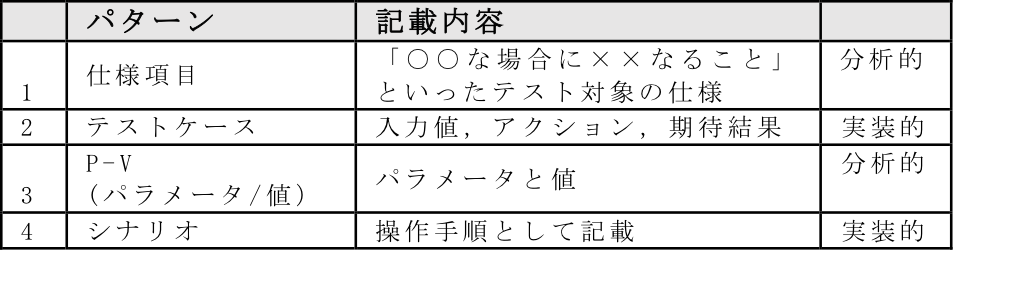
\includegraphics[width=7cm]{./image/D-3-Fig14.png}
  \caption{テスト分析パターン}
  \label{fig:D-3-Fig14}
  \end{center}
\end{figure}

今回のワークショップでは, e1a の演習にて,解答をこれまでの経験に基づいて自由に書いてもらうようにした.この結果, テストの記載パターンが4 つに分類できることがわかった.
%<表3 テスト記述パターン>
% Table generated by Excel2LaTeX from sheet 'Sheet4'
\begin{table}[htbp]
  \centering
  \caption{テスト記述パターン}
    \begin{tabular}{|c|p{8.57em}|p{10.215em}|p{3.855em}|}
    \hline
          & \textbf{パターン} & \textbf{記載内容} & \multicolumn{1}{c|}{} \bigstrut\\
    \hline
    1     & 仕様項目  & 「○○な場合に××なること」といったテスト対象の仕様 & 分析的 \bigstrut\\
    \hline
    2     & テストケース & 入力値,アクション,期待結果 & 実装的 \bigstrut\\
    \hline
    3     & P-V
(パラメータ/値) & パラメータと値 & 分析的 \bigstrut[t]\\
    4     & シナリオ  & 操作手順として記載 & 実装的 \bigstrut[b]\\
    \hline
    \end{tabular}%
  \label{tbl:D-3-tbl11}%
\end{table}%

この4パターンとテスト条件の特定数に相関があるかをスピアマンの順序相関分析を使って調べたが,相関があると結論付けられる値にはならなかった.

これらの実験結果から特定の要因は見出せなかったが,それぞれの分析方法のばらつきから起きる重複や欠落の課題は現象として確認できた.

表~\ref{tbl:D-3-tbl11}の1 と3 は中間成果物的であり, 記載した内容を見てそのままテストを実行するには不向きである.一方,2と4 はそのままテスト実行時に利用できる. 一方, 分析や設計をすると1 と3 が成果物になる.自由に記載してもらう際に分析結果から書くことは,普段の業務でも分析や設計をしていると想定できる. なので, 2と4 を直接書くのは, 普段の業務であまり分析や設計行為をしていないのではないかという仮説を持った.仮説が正しければ, 普段から業務にて分析や設計をしている参加者のほうが, 慣れているために知識の習得が早いと想定し, 今回のワークショップを通じた演習結果にてこれまでの記載方法と演習の成果に相関があるかを調査した.図~\ref{fig:D-3-Fig13} がスピアマンの順序相関分析をした結果である, e1a では,仕様項目から記載する参加者と特定できたテスト条件数には, 0.51(0.4 以上の値は相関ありといえる)の相関が出たたがそれ以外は0.4 以上の値は出なかった.
グラフの傾向からは,e2では分析的な記述をしていた参加者のほうが実装的な記述をした参加者より正の相関となったが, 分析結果の値は0.2 をきっているため,相関があるとは結論付けられない.
\begin{figure}[h]
  \begin{center}
  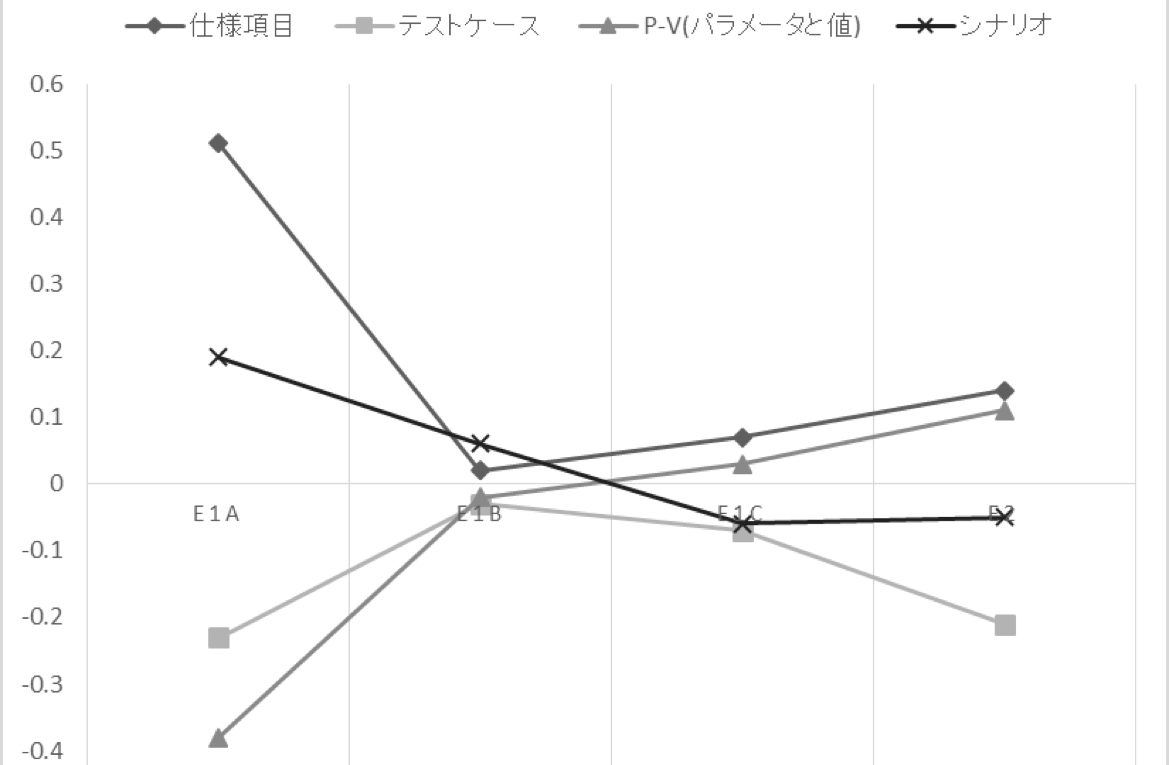
\includegraphics[width=10cm]{./image/D-3-Fig13.png}
  \caption{e1aの参加者業務分野別テスト条件特定数}
  \label{fig:D-3-Fig13}
  \end{center}
   \end{figure}


これらの検証実験にて,本手法の説明を参加者にすることによる仕様項目の一貫性と特定する量の向上が観察できた.更にI/Oデータパターンを使った実験結果の分析によって,実験結果の一部が本手法で提唱している仮説と一致することを観察できた.更に高精度に傾向を分析するため,更なる検証実験は必要である.以降のこの手法の効果と関連する要因とその傾向に対する深い理解とそのための更なる実験をすることで,AUTとフォールトの知識をベースにしたテストカテゴリを作るためのルールをより洗練できると考えている.

e1a の仕様項目を記載する参加者だけ相関が出たのは,今回の演習で特定するテスト条件が仕様項目そのものであるため,最初の演習では仕様項目を記載した参加者と結果の相関が出たと考えられる.

\newpage
\section{まとめ}
